\noindent\makebox[\linewidth][c]{学号：\underline{\hspace{9em}}\qquad 姓名：\underline{\hspace{9em}}}\par
\pdfbookmark[0]{一、填空题}{fillin}
\section{填空题（20 分）}
\begin{question}[index=1]
请写出以下问题是由哪一层协议解决的：（1）在 \underline{\hspace{4em}} 层决定数据报的路径；（2）在 \underline{\hspace{4em}} 层把传输的位流分成数据帧；（3）在 \underline{\hspace{4em}} 层将光脉冲变换为二进制码。
\end{question}
\begin{question}[index=2]
Ping 命令是利用（4）\underline{\hspace{5em}} 报文来测试目的端主机的可达性。
\end{question}
\begin{question}[index=3]
（5）\underline{\hspace{5em}} 路由协议是典型的距离向量算法，（6）\underline{\hspace{5em}} 路由协议是链路状态算法。
\end{question}
\begin{question}[index=4]
对于某带宽为 4kHz 的低通信道，采用 16 种不同的物理状态来表示数据，假设无噪音，信道的最大传输速率是（7）\underline{\hspace{6em}}。
\end{question}
\begin{question}[index=5]
100Base-T 使用（8）\underline{\hspace{6em}} 作为传输媒体。
\end{question}
\begin{question}[index=6]
PPP 帧用 SONET 链路传输时，接收端收到的 PPP 帧的数据部分是 0001110111110111110110，问删除发送端加入的零比特后，原始发送的数据部分为（9）\underline{\hspace{8em}}。
\end{question}
\begin{question}[index=7]
要发送的原始数据是 10011010，若采用 CRC，生成多项式是 $P(X)=X^3+X^2+1$，则最终发送的数据为（10）\underline{\hspace{8em}}。
\end{question}
\begin{question}[index=8]
具有 5 个 10M 端口的集线器的总带宽可以达到（11）\underline{\hspace{5em}}，同样配置的以太网交换机的总带宽可达（12）\underline{\hspace{5em}}。
\end{question}
\begin{question}[index=9]
根据图 1 的路由表，目的地址为 128.9.25.9 的数据报应该送往（13）\underline{\hspace{6em}}。
\par\smallskip\noindent\makebox[\linewidth][c]{%
\begin{tabular}{|l|c|}\hline
Prefix & Port\\\hline
--- & ---\\\hline
128.9/16 & 5\\\hline
128.9.16/20 & 2\\\hline
128.9.19/24 & 7\\\hline
128.9.25/24 & 10\\\hline
128.9.176/20 & 1\\\hline
--- & ---\\\hline
\end{tabular}}
\par\noindent\makebox[\linewidth][c]{图 1}
\end{question}
\pdfbookmark[0]{二、简答题}{short}
\section{简答题（35 分）}
\begin{question}[index=1]
（8 分）请简述并对比电路交换和分组交换的异同。
\end{question}
\begin{question}[index=2]
（7 分）IPv6 向 IPv4 过渡的方法有哪些？请对其中一种方法进行说明。
\end{question}
\begin{question}[index=3]
（10 分）如图 2，A、B 是子网 1 中的主机，C 是子网 2 中的主机，简述 A-B 通信时与 A-C 通信时使用 ARP 协议的具体情况。
\par\noindent\makebox[\linewidth][c]{\begin{tikzpicture}[x=1cm,y=1cm,line width=.55pt,
  every node/.style={inner sep=2pt},
  network/.style={draw,rounded corners=2pt,minimum width=1.5cm,minimum height=.8cm},
  router/.style={draw,ellipse,minimum width=1cm,minimum height=.55cm,inner sep=0pt},
  host/.style={draw,minimum width=6mm,minimum height=6mm}]
\node[network] (N1) at (0,0) {网络 1};
\node[network] (N2) at (8.4,0) {网络 2};
\node[network] (N3) at (8.4,2) {网络 3};
\node[router] (R1) at (2.8,0) {$\times$};
\node[router] (R2) at (5.6,0) {$\times$};
\node[router] (R3) at (5.6,2) {$\times$};
\node[host] (A) at (-.5,-1.3) {A};
\node[host] (B) at (.5,-1.3) {B};
\node[host] (C) at (8.4,-1.3) {C};
\draw (N1.east)--(R1.west);
\draw (R1.east)--(R2.west);
\draw (R2.east)--(N2.west);
\draw (R2.north)--(R3.south);
\draw (R3.east)--(N3.west);
\draw (A.north)--(-.5,-.4);
\draw (B.north)--(.5,-.4);
\draw (C.north)--(N2.south);
\node[anchor=north] at (2.8,-.35) {R1};
\node[anchor=north] at (5.6,-.35) {R2};
\node[anchor=south] at (5.6,2.35) {R3};
\node[anchor=north] at (2.05,-.05) {e0};
\node[anchor=north] at (3.55,-.05) {e1};
\node[anchor=north] at (4.85,-.05) {e2};
\node[anchor=north] at (6.35,-.05) {e3};
\node[anchor=east] at (5.5,.55) {e4};
\node[anchor=east] at (5.5,1.45) {e5};
\node[anchor=north] at (6.35,1.95) {e6};
\end{tikzpicture}
}
\par\noindent\makebox[\linewidth][c]{图 2}
\end{question}
\begin{question}[index=4]
（10 分）请对比并阐述距离向量路由算法和链路状态路由算法的优缺点。
\end{question}
\pdfbookmark[0]{三、计算题}{calculation}
\section{计算题（45 分）}
\begin{question}[index=1]
（12 分）在一个 CSMA/CD 网络中，主机 A 和 B 距离为 2km，数据传输率为 10Mb/s，线缆上的信号传播速度为 200 000km/s。
\begin{enumerate}
\item 若主机 A 和 B 发送数据时产生冲突，则从开始发送数据的时刻起，到两台主机检测到冲突为止，最短需要经过多长时间？最长需要经过多长时间？
\item 若网络不存在任何冲突与差错，主机 A 总是以标准的最长以太网数据帧（1518 字节）向主机 B 发送数据，主机 B 每成功收到一个数据帧后立即向主机 A 发送一个 64 字节的确认帧，主机 A 收到确认帧后方可发送下一个数据帧。此时主机 A 的有效数据传输率是多少（不考虑以太网的前导码）？
\end{enumerate}
\end{question}
\begin{question}[index=2]
（18 分）如图 2 所示网络拓扑中，
\begin{enumerate}
\item 网络 1 由 100 台主机，网络 2 由 50 台，网络 3 有 20 台，请将 166.111.4.0/24 划分给子网 1、2、3，须给出各子网的前缀长度、各子网的网络号（网络地址）和广播号（广播地址），并写出路由器各端口的 IP。
\item 当 A 发送报文给 C，A$\to$R1、R1$\to$R2、R2$\to$C 三个过程中，写出各个报文的源 IP、目的 IP、源 MAC、目的 MAC（用 MAC-A、IP-A、MAC-e0 等表示）。
\item 假设主机 A 向主机 C 发送一个总长度为 1500B 的 IP 分组，网络 2 的 MTU=800B，路由器 R2 在转发该 IP 分组时进行了分片。至少需要分为几个分片？请列出每个分片的总长度字段值、片偏移字段值，以及 MF 标志位的值。
\end{enumerate}
\end{question}
\begin{question}[index=3]
（15 分）如图 3 给定的网络拓扑，（1）使用距离向量算法计算每个路由节点的路由表。（2）在路由收敛后，B 和 D 之间距离由 5 变为 50，请列出节点路由表变化情况。
\par\smallskip\noindent\makebox[\linewidth][c]{%
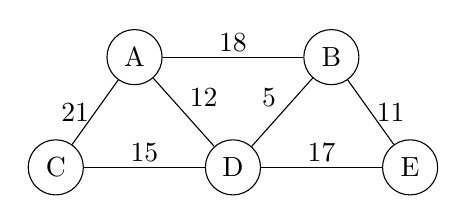
\begin{tikzpicture}[x=1cm,y=1cm,every node/.style={inner sep=2pt}]
\node[draw,circle,minimum size=7mm] (A) at (0,1.4) {A};
\node[draw,circle,minimum size=7mm] (B) at (2.5,1.4) {B};
\node[draw,circle,minimum size=7mm] (C) at (-1,0) {C};
\node[draw,circle,minimum size=7mm] (D) at (1.25,0) {D};
\node[draw,circle,minimum size=7mm] (E) at (3.5,0) {E};
\draw (A)--node[above]{18}(B);
\draw (A)--node[left]{21}(C);
\draw (A)--node[above right]{12}(D);
\draw (C)--node[above]{15}(D);
\draw (B)--node[above left]{5}(D);
\draw (B)--node[right]{11}(E);
\draw (D)--node[above]{17}(E);
\end{tikzpicture}}
\par\noindent\makebox[\linewidth][c]{图 3}
\end{question}
